\documentclass[../main.tex]{subfiles}

\begin{document}
    to procedury wywodzenia/wybierania przypadków testowych.
    \begin{itemize}
        \item systematyzują podejście do testowania
        \item efektywne w znajdowaniu możliwych awarii
        \item mogą uchronić przed redundantnymi testami
        \item powtarzalne
        \item oparte na modelach (np. działania oprogramowania)
        \item dostarczają elementy pokrycia
    \end{itemize}

    \begin{tabular}{|c|c|}
        \hline
        \textbf{Technika} & \textbf{Element pokrycia}\\
        \hline
        Podział na klasy równoważności & Klasa równoważności\\
        \hline
        Analiza wartości brzegowych & Wartości brzegowe\\
        \hline
        Drzewo klasyfikacji & Liść / kombinacja liści\\
        \hline
        Graf przyczynowo-skutkowy & Kombinacja przyczyn\\
        \hline
        Tablica decyzyjna & Kombinacja warunków\\
        \hline
        Testowanie maszyny stanowej & Przejście / sekwencja przejść\\
        \hline
        Graf przepływu sterowania & Ścieżka\\
        \hline
        CRUD & Cykl życia danej\\
        \hline
    \end{tabular}

    \textbf{Hipoteza błędu} - każda technika projektowania testów zaprojektowana jest do
    wykrywania określonego typu awarii.

    \textbf{Pokrycie} - stopień przetestowania elementów pokrycia dla zadanego
    warunku testowego, mierzone procentowo (0-100\%), dotyczy określonego kryterium.

    Zbiór testów spełnia kryterium pokrycia, jeśli pokrycie dla tych testów
    wynosi 100\%

    Kryterium K1 \textbf{subsumuje} kryterium K2, jeśli każdy zestaw testów
    spełniający K1 spełnia również K2.


    \subsection{Techniki projektowania testów}

    \begin{table}[H]
        \begin{center}
            \begin{tabular}{ p{5cm} p{5cm} p{5cm} }
                \toprule
                \textbf{oparte na specyfikacji} & \textbf{oparte na strukturze} & \textbf{oparte na doświadczeniu}\\
                \toprule
                specyfikacja używa
                modeli, formalnych
                lub nieformalnych
                &
                testy tworzone na
                podstawie informacji
                o strukturze programu
                &
                testy tworzone na
                podstawie wiedzy,
                doświadczenia i
                intuicji testerów\\

                przypadki testowe
                mogą być tworzone
                systematycznie z
                tych modeli
                &
                można mierzyć
                stopień pokrycia
                oprogramowania i
                dodawać nowe testy
                by zwiększyć pokrycie
                &
                inne źródło informacji
                to wiedza o
                możliwych defektach i
                ich umiejscowieniu\\

                \begin{itemize}
                    \item klasy równoważności
                    \item wartości brzegowe
                    \item tablice decyzyjne
                    \item grafy P-S
                    \item maszyna stanowa
                    \item drzewa klasyfikacji
                    \item przypadki użycia
                    \item testowanie losowe
                \end{itemize}
                &
                \begin{itemize}
                    \item pokrycie instrukcji
                    \item pokrycie decyzji
                    \item pokrycie warunków
                    \item pokrycie MC/DC
                    \item pokrycie przepływu danych
                    \item pokrycie pętli
                    \item pokrycie ścieżek
                    \item testowanie mutacyjne
                \end{itemize}
                &
                \begin{itemize}
                    \item t. eksploracyjne
                    \item zgadywanie błędów
                    \item ataki usterkowe
                    \item t. z listą kontrolną
                    \item testowanie ad hoc
                \end{itemize}\\
            \end{tabular}
        \end{center}
    \end{table}

    \textbf{Analiza wartości brzegowych}
    \begin{itemize}
        \item technika oparta na podziale na klasy równoważności
        \item działa dla klas, na których zadany jest porządek liniowy
        \item wartość brzegowa = wartość min/max zadanej klasy równoważności
        \item można rozważać wartości brzegowe dla wejścia i wyjścia
    \end{itemize}

    \textbf{Tablice decyzyjne}
    \begin{itemize}
        \item testowanie kombinacji warunków
        \item dobra metoda do testowania logiki biznesowej
        \item pozwala na systematyczne sprawdzanie wszystkich kombinacji
        \item ułatwia wykrywanie
        \begin{itemize}
            \item brakującej specyfikacji
            \item błędnej (sprzecznej) specyfikacji
        \end{itemize}
    \end{itemize}
    \textbf{Minimalizacja tablicy} - jeśli wszystkie kombinacje pewnych warunków dają te same akcje, możemy je scalić.

    \begin{table}[H]
        \begin{center}
            \begin{tabular}{p{8cm} p{8cm}}
                \textbf{Grafy przyczynowo-skutkowe}
                \begin{itemize}
                    \item stosowane w tych samych sytuacjach co tablice decyzyjne
                    \item graficzna reprezentacja zależności między przyczynami a skutkami
                    \item prosta transformacja na tablice decyzyjne
                \end{itemize}
                &
                \begin{figure}[H]
                    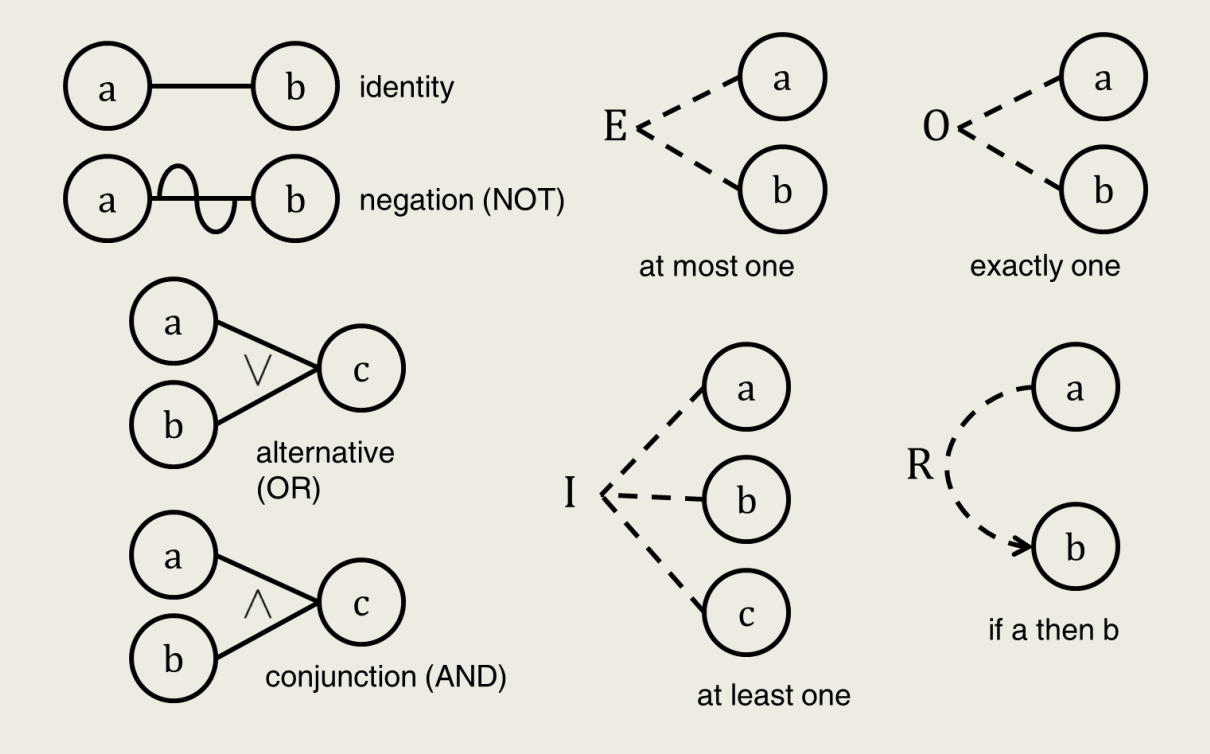
\includegraphics[width=0.5\linewidth]{graf.png}
                \end{figure}\\
            \end{tabular}
        \end{center}
    \end{table}

\end{document}